\chapter{ORIENTAÇÃO A OBJETOS}
\label{orientacaoAObjetos}

A orientação a objetos traz uma nova forma de se pensar a construção de sistemas
computacionais. Pois, diferentemente do pensamento em que se tinha durante a 
programação estruturada, onde eram definidos pequenos trechos de código sem que 
houvesse um contexto para agrupá-los, este novo paradigma faz com que os sistemas 
sejam construídos de maneira organizada, uma vez que trabalhamos com estruturas 
semelhantes as que conhecemos do nosso dia a dia
\cite{phpProgramandoComOrientacaoAObjetos}.

A orientação a objetos nos permite associar valores e funções em uma única
unidade: o objeto. Ao invés de termos variáveis com prefixos que indiquem o 
motivo de sua existência, ou valores armazenados em matrizes para manter os 
elementos juntos, com o uso de objetos podemos adicionar funcionalidades e 
comportamentos a uma unidade de software criando um novo tipo de dados: as 
classes \cite{phpMasterWriteCuttingEdgeCode}.

\section{CLASSE}

A classe é uma estrutura que agrupa as propriedades e os métodos de forma
abstrata com base no modelo de negócio do software que será desenvolvido. 
Sendo assim, é uma estrutura estática que agrupa de maneira lógica e descreve 
propriedades e métodos com base no modelo de negócio representando uma abstração 
da realidade \cite{phpProgramandoComOrientacaoAObjetos}.

Por conta disto, uma classe pode ser considerada como um modelo ou
\textit{template}, no qual, com base nesses modelos podem ser criados vários objetos.

Em uma analogia com o processo de preparação de um bolo, temos a classe como
sendo a receita e o objeto como o bolo. Onde, com base em uma receita podemos fazer 
vários bolos.

Para \citeonline{c++Absoluto}, uma classe é um novo tipo de dados assim como os já
existentes tipos primitivos: \textit{int} e \textit{double}, portanto, um método
ou uma variável podem usar uma classe ao trocarem mensagens, sendo assim a classe 
poderia ser utilizada como dado de entrada ou saída.

Portanto, as classes são os blocos de construção de uma aplicação, que quando
unidos dão origem a um software \cite{learningJava}. Sendo que, pode ser 
composta por: métodos, propriedades, códigos de construção e destruição, 
utilizando conceitos de: herança, polimorfismo, encapsulamento, interfaces e 
exceções. E por fim, um conjunto de classes poderá ser agrupado em um pacote.

\begin{figure}[h!tb]
	\centering
	\caption{Definição de uma Classe na linguagem PHP}
	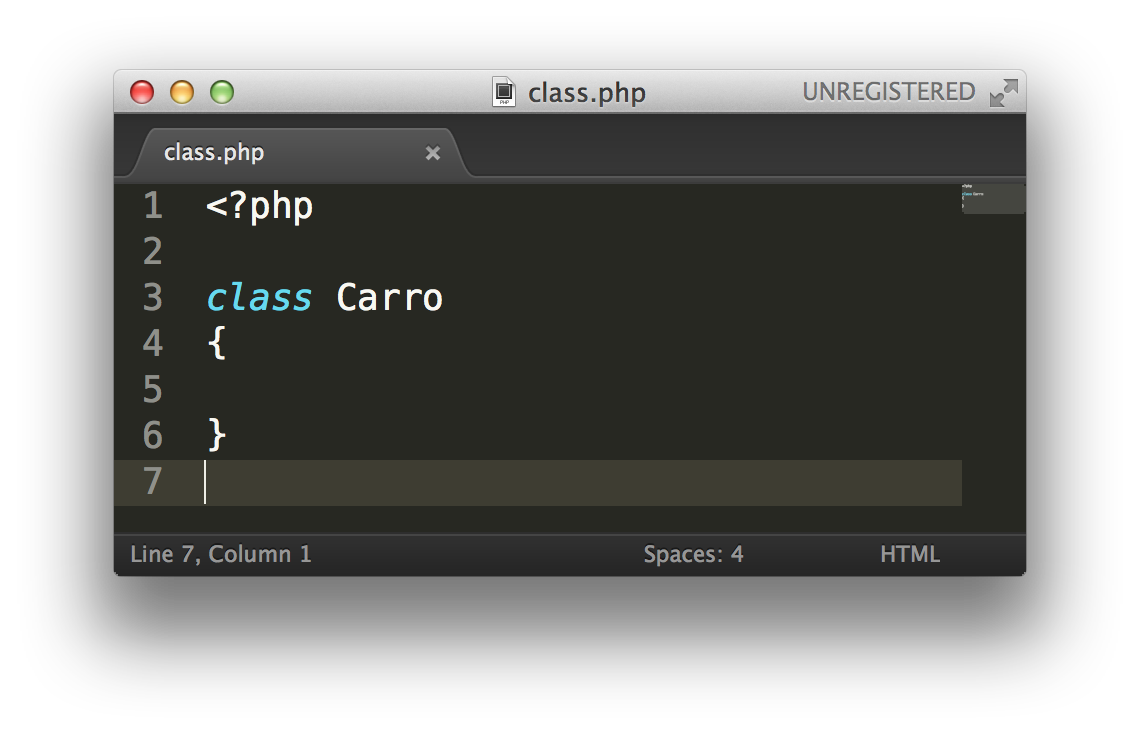
\includegraphics[width=\textwidth]{images/class.png}
	\label{fig:classe}
	\centering
	\footnotesize Fonte: \fonteOAutor
\end{figure}

\FloatBarrier 	% Este comando impede que as imagens 
				% flutuem a partir deste ponto no seu documento

Logo abaixo será apresentada a análise do código exibido na
figura \ref{fig:classe}:

\begin{enumerate}[a)]
    \item \textbf{linha 1:} temos o início da execução de um bloco de código
    PHP;
    \item \textbf{linha 3:} informamos ao interpretador da linguagem PHP que 
    estamos definindo um novo tipo de dados (uma nova estrutura) que será 
    identificada através do nome "Carro";
    \item \textbf{linha 4:} o símbolo \textbf{\{} se refere a abertura de um
    bloco de código, ou seja, informa ao interpretador onde inicia-se a definição de 
    características ou dados (propriedades ou atributos) e ações (métodos). 
    Ambos os conceitos métodos e propriedades veremos ao decorrer deste
    capítulo;
    \item \textbf{linha 6:} o símbolo \textbf{\}} se refere ao fechamento de um
    bloco de código, ou seja, informa ao interpretador onde terminam as
    definições de propriedades e métodos.
\end{enumerate}
\subsection{Objeto}

Um objeto é uma estrutura dinâmica construída com base em uma classe. Sendo que,
com base em uma classe é possível criar vários objetos, cada qual com suas
propriedades \cite{phpProgramandoComOrientacaoAObjetos}.

De forma breve, os objetos são as instâncias de uma classe. Sendo que, as
classes existem somente no código fonte de uma aplicação, enquanto que, as
instâncias de uma classe existem durante a execução de um programa. Portanto,
o software poderá criar vários objetos sob demanda tendo como base um mesmo
modelo \cite{ios7ProgrammingFundamentalsObjectiveCXcodeAndCocoaBasics}. Deste
modo, esses objetos são criados (instanciados) através de métodos construtores
e destruídos (eliminados) através de métodos destrutores em tempo de execução
\cite{umlEC++GuiaPraticoDeDesenvolvimentoOrientadoAObjeto}. Será apresentado no
decorrer deste capítulo como funcionam os métodos construtores e destrutores.

\begin{figure}[h!tb]
	\caption{Criação de um objeto na linguagem PHP}
	\label{fig:objeto}

	\centering
	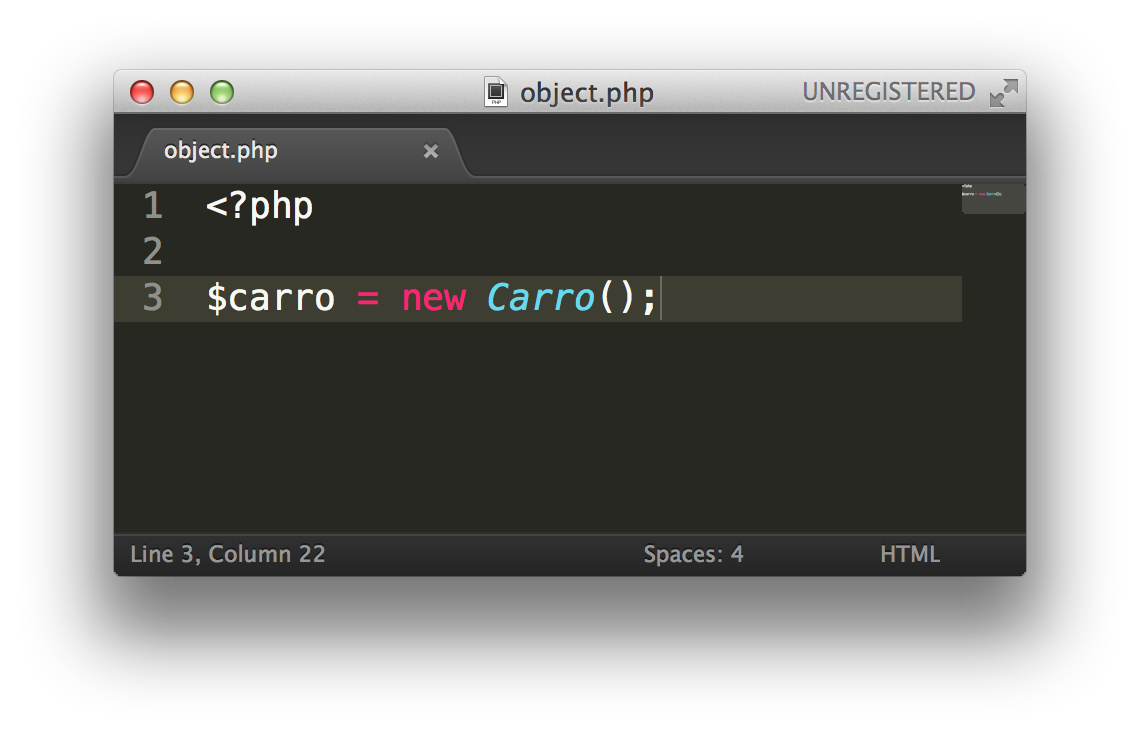
\includegraphics[width=0.65\textwidth]{images/object.png}

	\centering
	\footnotesize Fonte: \fonteOAutor
\end{figure}

\FloatBarrier 	% Este comando impede que as imagens
				% flutuem a partir deste ponto no seu documento

A seguir, será apresentada a análise do código exibido na
Figura \ref{fig:objeto}:

\begin{alineas}
    \item linha 1: tem-se o início da execução de um bloco de código PHP;
    \item linha 3: é definida uma variável chamada \textbf{\$carro};
    chama-se um operador de atribuição da linguagem (representado pelo símbolo
    \textbf{=}) que irá atribuir o valor que está à direita do operador na
    variável que está à esquerda; em seguida é informado um outro operador da
    linguagem (representado pelo símbolo \textbf{new}) que é responsável por
    criar uma referência em memória para o tipo de dados que está sendo
    criado e, por fim, define-se a classe que deverá ser instanciada, que neste
    caso, chama-se Carro. Logo após, o símbolo \textbf{()} representa um método
    construtor (conceito que será apresentado ainda neste capítulo de Orientação
    a Objetos).
    Uma informação importante é que toda instrução da linguagem \acs{PHP} termina
    com o símbolo de ponto-e-vírgula.
\end{alineas}
\subsection{Método}

Segundo \citeonline{php5ConceitosProgramacaoEIntegracaoComBancoDeDados}, um
método pode ser definido como sendo as operações que manipulam os dados de uma
classe, ou seja, definem o que as classes podem e sabem fazer, como por exemplo
acelerar um carro modificando o valor de sua propriedade chamada
\textit{velocidade} para um valor crescente em um determinado espaço de tempo.

Os métodos também podem ser chamados de funções membro \cite{c++ComoProgramar}.

Se comparado a programação estruturada um método pode ser considerado como sendo
uma função que está associada a uma classe \cite{programmingPhp}.

\begin{figure}[h!tb]
	\caption{Criação de um Método utilizando a linguagem PHP}
	\label{fig:metodo}

	\centering
	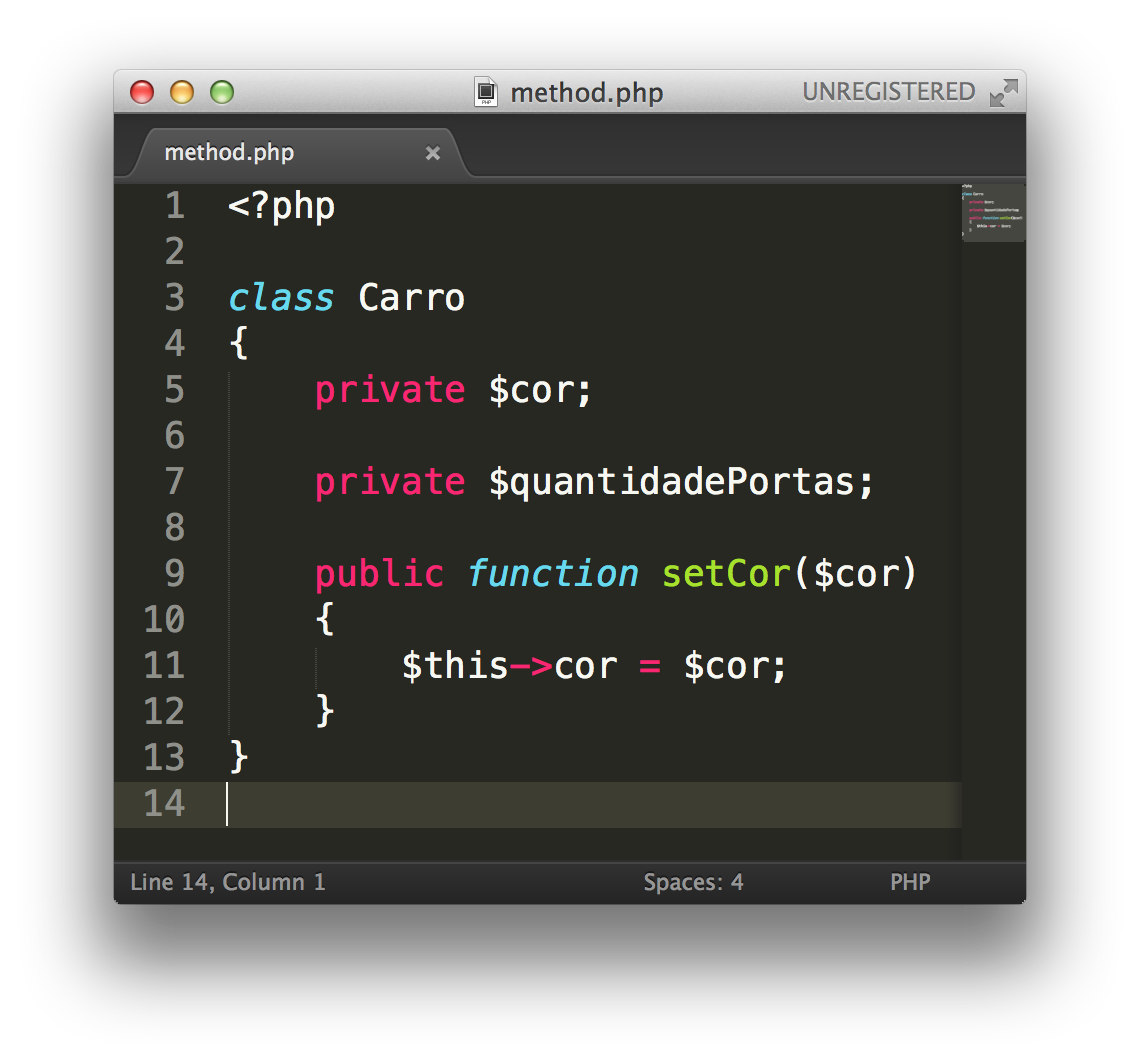
\includegraphics[width=0.68\textwidth]{images/method.png}

	\centering
	\footnotesize Fonte: \fonteOAutor
\end{figure}

\FloatBarrier 	% Este comando impede que as imagens
				% flutuem a partir deste ponto no seu documento

Na sequência, você irá conferir uma explicação referente ao código que foi
apresentado na Figura \ref{fig:metodo}:

\begin{enumerate}[a)]
    \item linha 1: vê-se o início da execução de um bloco de código PHP;
    \item linha 3: define-se uma classe chamada \textit{Carro};
    \item linha 4: informa-se onde inicia o bloco de uma classe;
    \item linha 5 e 7: cria-se duas propriedades para a classe
    \textit{Carro};
    \item linha 9: é solicitado para que o interpretador crie um método
    cuja visibilidade seja pública e define-se que este método será identificado
    pelo nome \textbf{setCor}.
    Além disso, informa-se que este método deve receber um parâmetro (um valor
    que  irá configurar a propriedade de uma classe);
    \item linha 10: define-se onde inicia o bloco cujo escopo
    corresponda ao método \textbf{setCor};
    \item linha 11: utilizou-se uma variável especial chamada
    \textbf{\$this}, esta variável permite acessar qualquer propriedade ou
    método dentro da própria classe ou \textit{superclasse}; depois, usou-se
    o operador de acesso a um objeto (representado pelo símbolo \textbf{->}); em
    seguida, informa-se ao interpretador do \acs{PHP}, a necessidade de
    manipular o valor da propriedade \textit{cor}, sendo que, ela deverá receber o valor
    informado como parâmetro para o método \textbf{setCor};
    \item linha 12: define-se onde termina o bloco que corresponde ao
    método \textbf{setCor};
    \item linha 13: informa-se o encerramento do bloco de uma classe.
\end{enumerate}

Como foi visto o conceito de métodos a seguir será apresentado o conceito de
propriedades.

\subsection{Propriedade}

Assim como a comparação realizada anteriormente, que abordou o que é um método
comparando-o com os conceitos da programação estruturada, seguindo a mesma
analogia, uma propriedade (também conhecida como atributo, variável membro ou ainda variável
de instância) pode ser considerada como os dados que um objeto possuí,
descrevendo desta forma, as características que a ele pertencem
\cite{programmingPhp}.

Sendo assim, os atributos são variáveis que estão definidas dentro de uma
classe, deste modo, geralmente são acessados através de uma interface de acesso,
pois não estão visíveis para que outros objetos manipulem os dados diretamente,
se isto ocorresse, poderia comprometer a segurança da informação e também o
conceito de que cada objeto possuí uma finalidade.

Então, uma propriedade (pensando na classe Carro) poderia ser uma característica
que um carro possuí no mundo real. Portanto, é possível levantar de acordo com
o nosso conhecimento rapidamente os seguintes parâmetros que definem um carro:
cor, quantidade de portas, possuí direção hidráulica, etc.

Na Figura \ref{fig:propriedade}, é apresentada a sintaxe para definição de duas
propriedades (cor e quantidade de portas) da classe Carro implementadas na
linguagem \acs{PHP}.

\begin{figure}[h!tb]
	\caption{Criação de propriedades na linguagem PHP}
	\label{fig:propriedade}

	\centering
	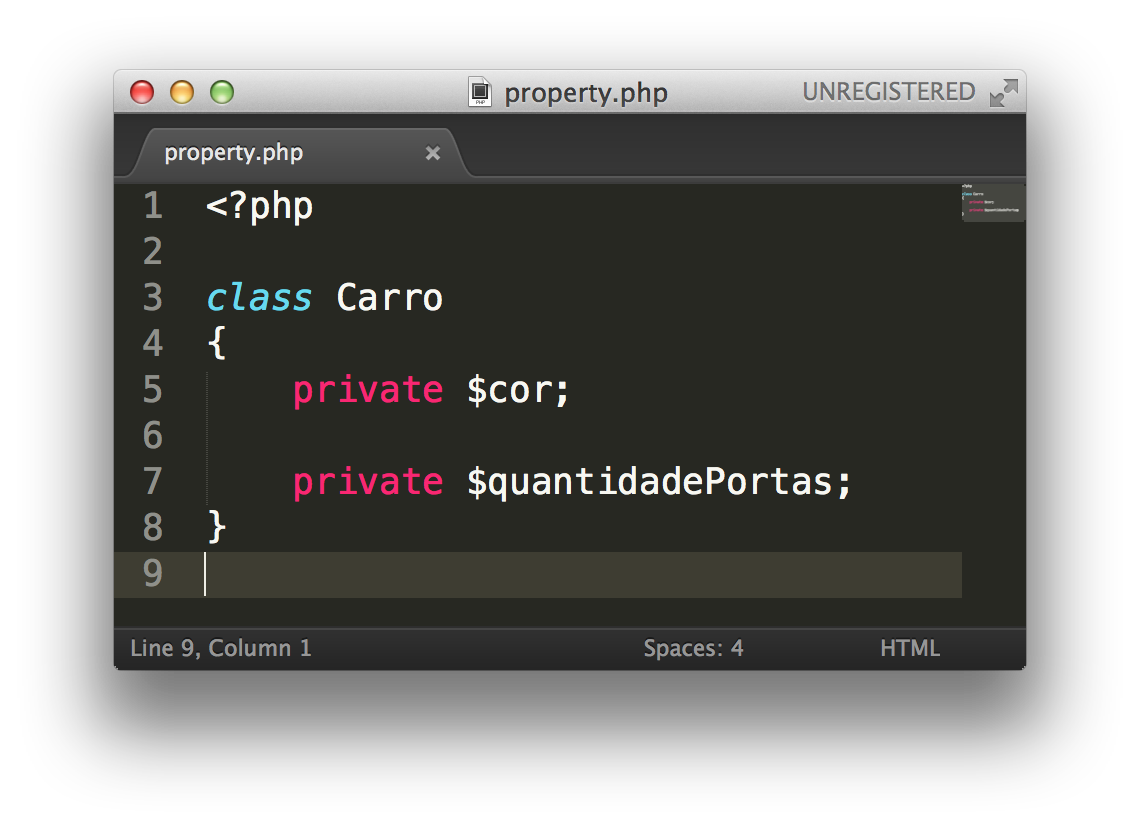
\includegraphics[width=0.75\textwidth]{images/property.png}

	\centering
	\footnotesize Fonte: \fonteOAutor
\end{figure}

\FloatBarrier 	% Este comando impede que as imagens
				% flutuem a partir deste ponto no seu documento

Por conseguinte, abaixo será apresentada a análise das linhas de código
exibidas na Figura \ref{fig:propriedade}:

\begin{alineas}
    \item linha 1: vê-se o início da execução de um bloco de código PHP;
    \item linha 3: define-se uma classe chamada \textit{Carro};
    \item linha 5: utiliza-se uma palavra reservada \textbf{private} que se
    refere a visibilidade da propriedade no contexto de um conjunto de objetos
    (mais detalhes serão apresentadas adiante) e, em seguida, é definido o nome
    de uma variável, que neste caso chama-se \textbf{\$cor};
    \item linha 7: é definida uma segunda propriedade para a classe
    Carro chamada de \textbf{\$quantidadePortas};
    \item linha 8: informa-se onde termina o bloco que compreende a
    classe \textit{Carro}.
\end{alineas}

\subsubsection{Propriedade estática}

Como foi visto anteriormente, as classes são formadas por variáveis de instância
e métodos. Entretanto, as variáveis que forem declaradas com a palavra reservada
\textit{static}, serão compartilhadas por toda a classe. Por conta disto, as
variáveis que assim forem definidas, recebem o nome de variáveis estáticas ou ainda
propriedades estáticas \cite{learningJava}.

Conforme afirma \citeonline{c++ComoProgramar}, a palavra chave \textit{static}
é utilizada quando as informações precisam ser compartilhadas por todas
as instância e não apenas em um único objeto.

Na Figura \ref{fig:propriedadeEstatica} é exibido um exemplo de propriedade
estática utilizando a linguagem \acs{PHP}.

\begin{figure}[h!tb]
	\caption{Propriedade estática definida na linguagem PHP}
	\label{fig:propriedadeEstatica}

	\centering
	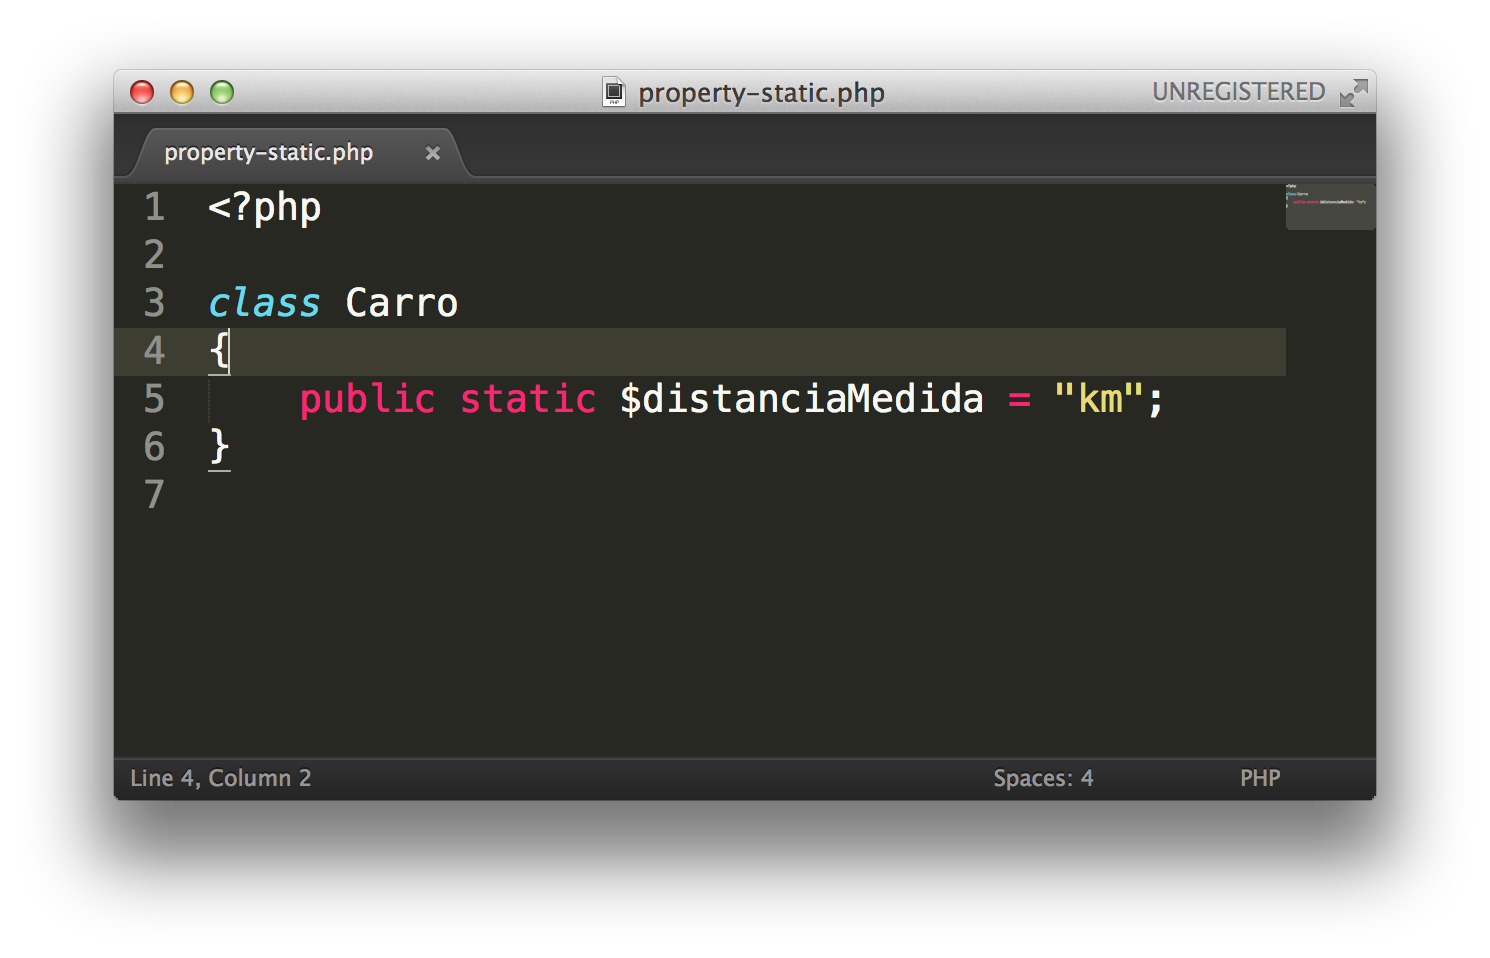
\includegraphics[width=0.82\textwidth]{images/property-static.png}

	\centering
	\footnotesize Fonte: \fonteOAutor
\end{figure}

\FloatBarrier 	% Este comando impede que as imagens
				% flutuem a partir deste ponto no seu documento

A seguir, é apresentado em detalhes as linhas de código exibidas na Figura
\ref{fig:propriedadeEstatica}:

\begin{alineas}
    \item linha 1: vê-se o início da execução de um bloco de código PHP;
    \item linha 5: define-se a propriedade estática que armazenará a unidade de
    medida utilizada por todos os veículos, que neste caso é \textit{km}
    (quilômetros).
\end{alineas}

A seguir será apresentado o conceito que define o que é uma constante e
exibido um exemplo de uso implementado na linguagem \acs{PHP}.
